\subsubsection{Individual Permissions}

For the purposes of this section, an individual refers to an individual identity. This may be held by an organisation or by a person, and is someone to whom the data owner directly gives permissions.

There are several considerations to make when giving another identity permissions:

\begin{itemize}
  \item 
  	\textbf{Access Control} \\
    The ability of an individual to get access to the location of a file
  \item
  	\textbf{Read} \\
    The ability of an individual to read the contents of a file, correctly.
  \item
    \textbf{Write} \\
    The ability of an individual to write the contents of a file, correctly.
\end{itemize}

\paragraph{Access Control}

A simple permissions system based on basic UNIX ACL (access control list) permissions is used, allowing a number $x$ in the range of $[0..2^n)$ where $n$ represents the number of permission types available (read, write, etc.). $x$ models the permissions for a given identity. This project only requires primitive permissions to show proof of concept, those permissions being only 'read' and 'write'. Given these two possibilities there are four possible permission settings per identity:

\begin{table}[H]
  \centering
  \begin{tabular}{ | l | c | c | }
    \hline
    Number & Read & Write \\
    \hline
    0 & & \\
    1 & \checkmark & \\
    2 & & \checkmark \\
    3 & \checkmark & \checkmark \\
    \hline
  \end{tabular}
  \caption{
  	Identity permission modeling
  }{
    The four possible permissions settings an identity could have at any given time. Each setting is mutually exclusive of any other.
  }
  \label{table:pre_properties}
\end{table}

Given the settings in table it is easy to understand whether any identity has a given permission. Let's imagine a system that has $n = 20$, and we wish to understand if a particular identity, with permissions $x$, has permission $14$ set. We apply the following function:

\begin{figure}[H]
  \centering
  \begin{minted}{haskell}
hasPermission :: (Num a, Bool b) => a -> a -> b
hasPermission 0 _                = false
hasPermission x p | x < 2**(p-1) = false
                  | otherwise    = x mod (2**p) > (2**(p - 1))
  \end{minted}
  \caption{
  	Permissions check for a given $n$
  }{
  	$x$ represents the permissions for a given user. $p$ represents the permissions bit we wish to check for.
  }
  \label{code:storage_permissions_check}
\end{figure}


The function shown in figure \ref{code:storage_permissions_check} is derived from the fact that a permission $n$ is represented by the $n-1^{\text{th}}$ bit, such that if all possible permissions were set for a given user, $x = 2^{n} - 1$. 

\paragraph{Read}

As part of the storage contract deployed, a function must be available returning a reference to the public key of the storage contract owner, which can then be retrieved from off-chain storage. Intuitively, no security is required in terms of the storage of this public key.

When an individual is given read access, it is important to consider how they will read the contents of the encrypted data (only decrypt-able by the storage contract owner). Since the public key of any individual registered is available through their storage contract, the storage contract owner is able to use the individual's public key and their local copy of their private key to generate a re-encryption key. This re-encryption key is added at the point when an individual is granted read access. The reference to this key is available only as long as the individual has read access.

\begin{figure}[H]
  \centering
  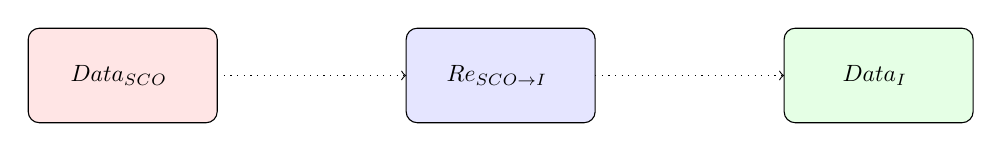
\begin{tikzpicture}[scale = 0.6, every node/.style={scale = 0.85}, every node/.append style={fill = white, rounded corners = 2pt, inner sep = 2pt, align = center}]

  \draw [rounded corners, fill=green!10] (6, 1) rectangle (10, -1);
  \node [fill=green!10] at (8, 0) { $\text{Data}_{\text{I}}$ };

  \draw [ -> , dotted] (2, 0) -- (6, 0);

  \draw [rounded corners, fill=blue!10] (-2, 1) rectangle (2, -1);
  \node [fill=blue!10] at (0, 0) { $\text{Re}_{\text{SCO} \rightarrow \text{I}}$ };

  \draw [ -> , dotted] (-6, 0) -- (-2, 0);

  \draw [rounded corners, fill=red!10] (-6, 1) rectangle (-10, -1);
  \node [fill=red!10] at (-8, 0) { $\text{Data}_{\text{SCO}}$ };

  \end{tikzpicture} \\
  \caption{
  	Individual Read Re-encryption
  }{
    The process of taking data encrypted for a storage contract owner, re-encrypting it from the storage contract owner to the individual, and then processing the resulting data as the individual (decryption).
  }
  \label{fig:encryption_individual_read}
\end{figure}


\paragraph{Write}

Other than the necessary write permission, an individual needs to possess the public key of the storage contract owner in order to appropriately encrypt all data. Any data which is referenced by the storage contract should be encrypted such that only the data owner is able to decrypt it without further re-encryption.
